\section{Dafny VSCode}
Github Repository: \href{https://github.com/FunctionalCorrectness/dafny-vscode}{https://github.com/FunctionalCorrectness/dafny-vscode}

\subsection{Overview}
\todo{Maybe add a class diagram}

\subsection{Visual Studio Code Plugin}
\subsubsection{Structure}
When a Visual Studio Code plugin is implemented as a language server, the plugin consists of two parts. The first one is an IDE-agnostic language server, which is further explained in \ref{langServer}. The second part is the actual plugin which interacts with Visual Studio Code and relies on the language server to provide functionality. \newline
The actual plugin will further on be referenced as the client part of the plugin. The most important part of the client part is a file called package.json. It informs the IDE about the following points:
\paragraph{Activation}
Details for what the plugin is designed and when it is activated. Normally, plugins stay dormant until a use case is triggered for which they are needed. For this project, this is the case whenever a Dafny file is opened in Visual Studio Code.

\paragraph{Commands}
Details which commands this plugin exposes. Next to standard callbacks such as when a file is first opened or saved, additional custom commands can be registered here. This projects exposes some custom commands such as to install the Dafny server or check the version of the server currently installed. This also includes key bindings for the registered commands.

\paragraph{Configuration}
Is used to configure a plugin. For this project this for instance entails the path to the Dafny executable or if it is running on a .NET or mono environment. It also sets Visual Studio Code specific configuration, such as how long of a delay should follow typing before the file is reevaluated.

\paragraph{Dependencies}
Details all the dependencies in the form of node modules that the plugin has.

\paragraph{Meta information}
Additionally, this section details meta information about the plugin such as who developed it, which version it has and so on.


\todo{Further explanation about the client side of the plugin}


\subsection{Language Server}

VS-Code Plugins can be implemented in two ways: the first one is via the standard VS-CODE API and the second one is in form of a language server. Language servers follow a standard protocol to provide services for working with different programming languages and offer often used features such as go to definition. While this offers great portability and easy integration with other IDEs or tools that work with language server, the implementation as a language server was rejected in this project. \newline
The main reason is that the project extends an existing plugin, which was already built around the standard VS-CODE API. After a phase of research and writing a small prototype it was decided that rewriting the plugin as a language server was not a feasible in regard to the work needed to be done compared to the project scope. \newline
A second consideration when making this decision was that the usage of language servers in VS-CODE plugins is very sparse at the moment. The big language integrations like typescript or javascript do not implement their plugins as language servers, while the golang plugin offers experimental support at this time. The not wide spread usage in this environment was therefore another reason to not implement a language server.


Server here refers to the Language Server and not the DafnyServer. The later one is explicitly written as DafnyServer.

\subsubsection{Communication Types}
There are two different types to communicate between the client and the server. It's either a notification or a request. 

\paragraph{Notification}
A notification is just a message which can be sent in both directions. But you can't wait for an answer. These types of messages are mostly used to inform the partner that something happened. 

\paragraph{Request}
A request on the other side is message, which will be answered.  

\subsubsection{Commands}
Commands are specified in the client and can trigger different actions. You can specify names for them and register shortcuts from them. Also the server can send commands. 

\subsubsection{Communication overview}
To get an overview over how the client and the server communicates, all the different notifications, requests and commands are explained. 


\subsubsection{Notification Server $\longrightarrow$ Client}

\textbf{ERROR}
This message is sent if something happens, which the user should be informed about. Like the compilation failed or the DafnyServer wasn't found. \newline

\textbf{WARNING}
This message is sent if the mono path is specified but mono is in the path. \newline

\textbf{INFO}
Info messages appear quite often to inform the user about the current progress. \newline

\textbf{queueSize}
This message updates the queue size number in the statusbar on the right side. \newline

\textbf{serverStarted}
This message contains two additional parameters, which are also important for the statusbar. Is the pid and the version of the started DafnyServer instance. It is sent after the dependencies have been checked and the DafnyServer have been spawn. \newline

\textbf{activeVerifiyingDocument}
As soon a verification is sent to the DafnyServer, the client is informed to show that, if the user has this file open. \newline

\textbf{verificationResult}
All verification results are sent to the server, for fast access times. Switching from one file to the other, updates the verification result on the left side based on these results. \newline

\textbf{changeServerStatus}
All states from the server are also sent to the client to update the statusbar. \newline

\textbf{ready}
This message is sent directly after the serverStarted message to inform the DafnyClientProvider that verification requests can now be sent. \newline

\subsubsection{Request Server $\longrightarrow$ Client}

\textbf{dafnymissing}
This informs the client that the verification of the DafnyServer has failed or that there is a newer version available. The text is sent as a additional parameter.  \newline

\subsubsection{Diagnostics Server $\longrightarrow$ Client}

\textbf{sendDiagnostics}
After a file has been verified the output is analyzed and errors are sent as diagnostics to the client. They contains also the message or even related locations, where the errors is coming from.  \newline

\subsubsection{Notification Client $\longrightarrow$ Server}

\textbf{verify}
This notification contains the document which has to be verified. On the server it is put into a queue and the result is sent via verificationResult. \newline

\subsubsection{Request Client $\longrightarrow$ Server}

\textbf{reset}
Resets the DafnyServer on the Server and restart it. Can be useful if the caching of the DafnyServer is not working correctly anymore. \newline

\textbf{compile}
Sends a request containing only the uri to the corresponding file. Starts the Dafny.exe with parameters to generate either a dll or a exe. After the compilation it returns possible errors, if it is executable and a message.\newline

\textbf{stop}
Stops the server and returns after the process has been terminated. This is used for the installation to be sure that the process is not run. \newline

\subsubsection{Commands Client}

\textbf{dafny.restartDafnyServer}
Restarts the DafnyServer with the "Reset Request".\newline

\textbf{dafny.installDafny}
First run the uninstallDafny command to be sure that there is no running instance. Afterwards downloads the latest version from GitHub. This process is either executed from an upgrade message, not installed message or can be executed manually. 
See \nameref{fig:Version upgrade available} for a better overview over the installation process. \newline

\textbf{dafny.uninstallDafny}
First stops any DafnyServer instance and deletes all files which belongs to Dafny. \newline

\textbf{dafny.showReferences}
This is used to show references from CodeLenses. Unfortunately the command editor.action.showReferences can not be used directly, because of some internal problems. To solve that, all parameters have to be copied and passed to this command. \newline

\textbf{dafny.editText}
Mainly used for all refactoring to chance text in the active text document. \newline

\textbf{dafny.compile}
\todo{add mac shortcut correctly}
Shortcut: ctrl+shift+b or %⇧⌘B 
\newline
Compile the current document \newline

\textbf{dafny.compileAndRun}
Shortcut: F5
\newline
Compile the current document and if there is a "Main Method" start the corresponding executable. \newline


\subsubsection{Startup process}
\begin{figure}[H]
	\centering
	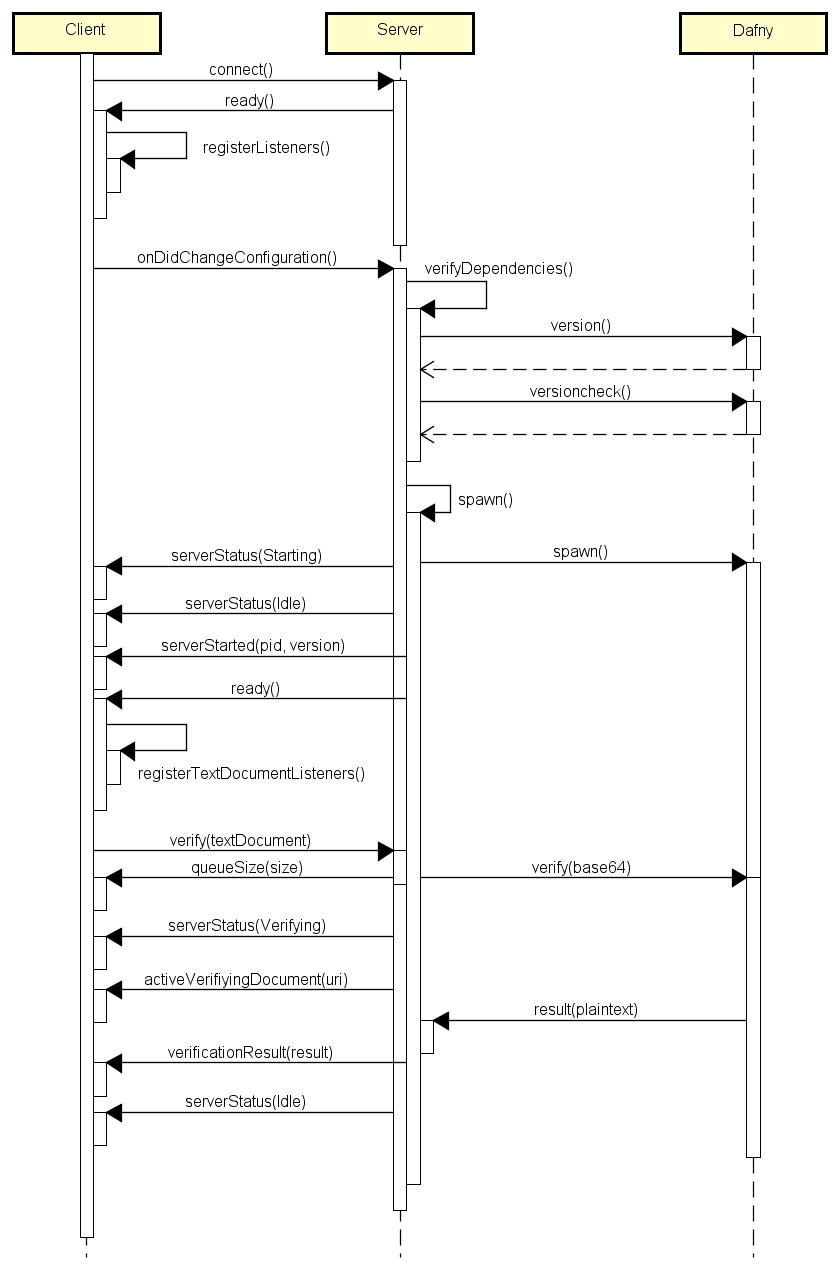
\includegraphics[width=1\textwidth]{img/DafnyStartupFull}
	\caption{DafnyServer startup}
	\label{fig:DafnyServer startup}
\end{figure}

\subsubsection{Not installed}
\begin{figure}[H]
	\centering
	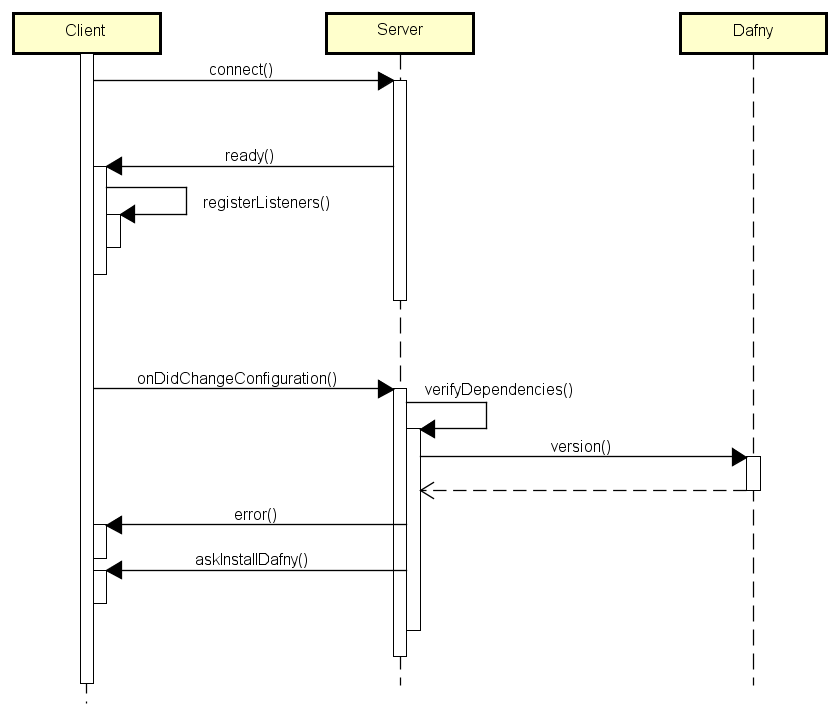
\includegraphics[width=1\textwidth]{img/DafnyNotInstalled}
	\caption{Dafny not installed}
	\label{fig:Dafny not installed}
\end{figure}

\subsubsection{Installation - Upgrade available}
\begin{figure}[H]
	\centering
	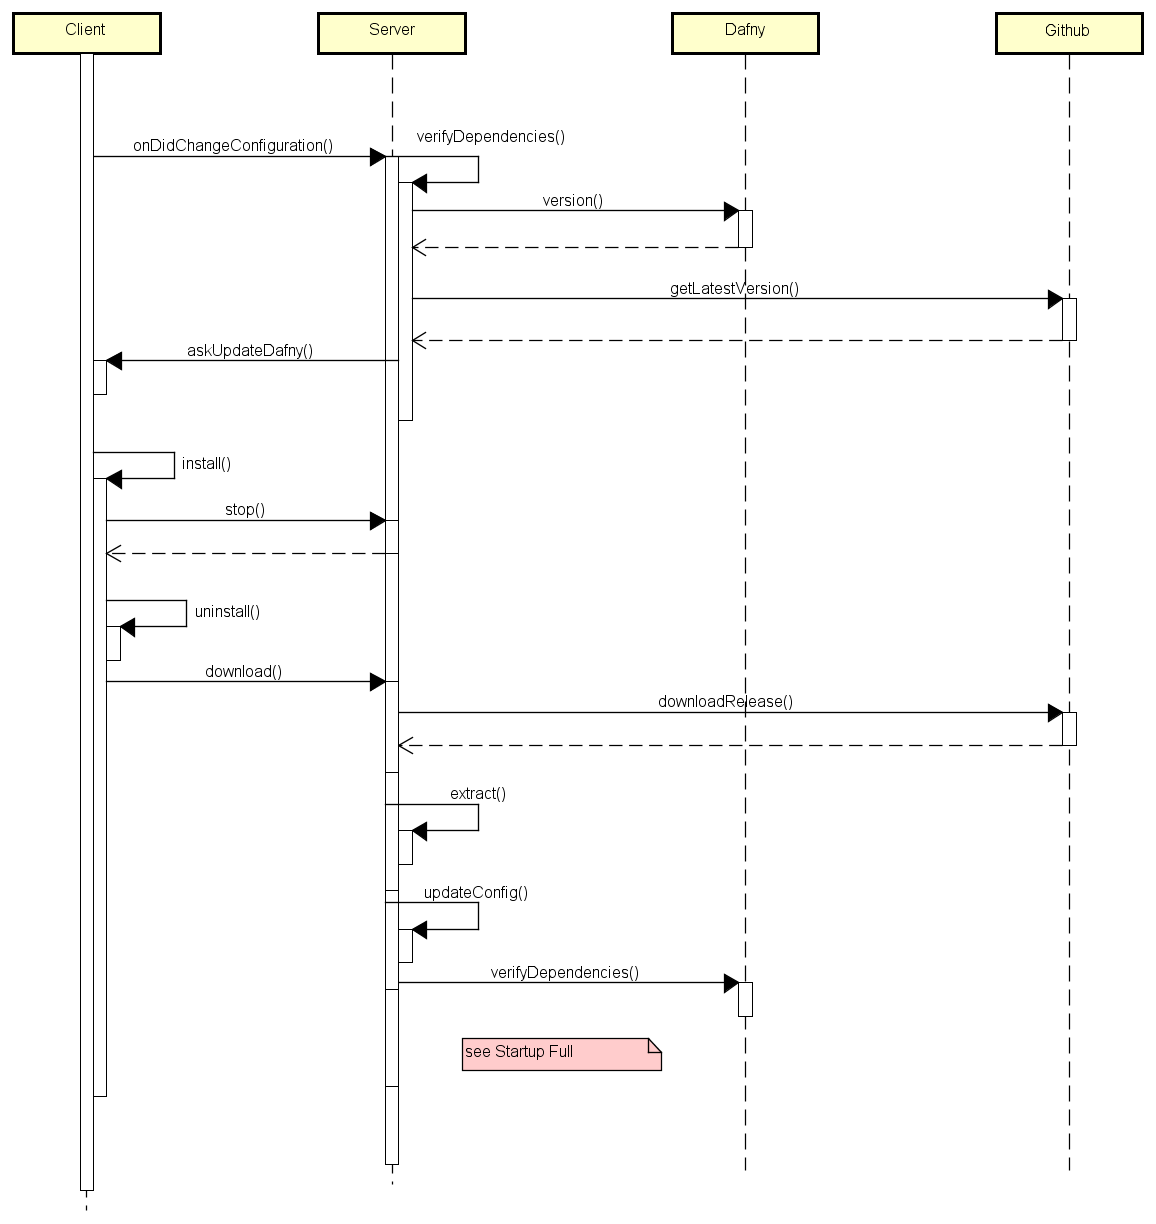
\includegraphics[width=1\textwidth]{img/DafnyVersionUpgrade}
	\caption{Version upgrade available}
	\label{fig:Version upgrade available}
\end{figure}





\subsection{Extension points}

\paragraph{Status bar}

\paragraph{Refactoring}

\paragraph{CodeLens}

\paragraph{Go to definition}

\subsection{Communication}

\subsection{Syntax highlighting}

\subsection{Snippets}

\subsection{Automatic installation}


\subsection{DafnyServer}
Github Repository: \href{https://github.com/FunctionalCorrectness/dafny-microsoft}{https://github.com/FunctionalCorrectness/dafny-microsoft}

The DafnyServer is a simple console application which allows proofing Dafny source files. To verify documents, they are sent over the standard input. Results are obtained from the standard output. The verification task needs to be in JSON format \todo{add reference to source.cs} and is sent base64 encoded. By default, the server only supports the verbs verify, quit and selftest. Verbs are sent first, followed by a newline \textbackslash{n}. They may be proceeded by a payload and an end string \textbf{[[DAFNY-CLIENT: EOM]]}. \newline 
Verb explanation: Verify needs a verification task and returns if all proofs holds, quit stops the server and selftest execute some simple verification. \newline

\textbf{Example verification task}
\begin{lstlisting}[language=json,firstnumber=1]
{
	args:[],
	filename:"c:\Users\Markus\Desktop\dafny\test1.dfy",
	source:"method Main() {	assert 1 < 3; }",
	sourceIsFile:false
}

\end{lstlisting}

\subsubsection{symbols}
To support refactoring in the Dafny Visual Studio Code plugin, symbol information was needed. All fields, methods and classes inside a file along with their information about position, reference and usage have to be accessible. To support this, the DafnyServer was extended. A new verb "symbols" was introduced. This collects various information about the symbol table of the input file and returns it as JSON. 
\newline\newline
\textbf{Request: }

\begin{lstlisting}[language=dafny]
class BankAccountUnsafe {
  var balance: int;
  constructor() modifies this { 
    balance := 10;
  }
  
  method withdraw(amount: int) 
    modifies this
    requires amount >= 0
  {   
    balance := balance - amount; 
  } 
}   

method test() { 
  var a := new BankAccountUnsafe(); 
  a.withdraw(9);  
}   
\end{lstlisting}

\textbf{Result: }
\begin{lstlisting}[language=json,firstnumber=1]
[ 
....
{
  "Call" : null,
  "Column" : 3,
  "EndColumn" : null,
  "EndLine" : null,
  "EndPosition" : null,
  "Ensures" : [],
  "Line" : 3,
  "Module" : "_module",
  "Name" : "_ctor",
  "ParentClass" : "BankAccountUnsafe",
  "Position" : 49,
  "References" : [{
    "Column" : 12,
    "Line" : 15,
    "MethodName" : "test",
    "Position" : 265,
    "ReferencedName" : "_ctor"
  }],
  "Requires" : [],
  "SymbolType" : "Method"
}, {
  "Call" : null,
  "Column" : 9,
  "EndColumn" : null,
  "EndLine" : null,
  "EndPosition" : null,
  "Ensures" : [],
  "Line" : 6,
  "Module" : "_module",
  "Name" : "withdraw",
  "ParentClass" : "BankAccountUnsafe",
  "Position" : 114,
  "References" : [{
    "Column" : 5,
    "Line" : 16,
    "MethodName" : "test",
    "Position" : 296,
    "ReferencedName" : "withdraw"
  }],
  "Requires" : ["amount >= 0"],
  "SymbolType" : "Method"
}, {
  "Call" : null,
  "Column" : 6,
  "EndColumn" : null,
  "EndLine" : null,
  "EndPosition" : null,
  "Ensures" : null,
  "Line" : 2,
  "Module" : "_module",
  "Name" : "balance",
  "ParentClass" : "BankAccountUnsafe",
  "Position" : 32,
  "References" : [{
    "Column" : 5,
    "Line" : 4,
    "MethodName" : "balance",
    "Position" : 85,
    "ReferencedName" : "balance"
  }, {
    "Column" : 3,
    "Line" : 10,
    "MethodName" : "balance",
    "Position" : 190,
    "ReferencedName" : "balance"
  }, {
    "Column" : 14,
    "Line" : 10,
    "MethodName" : "balance",
    "Position" : 201,
    "ReferencedName" : "balance"
  }],
  "Requires" : null,
  "SymbolType" : "Field"
}
.... 
]
\end{lstlisting}


\subsubsection{version}
The command returns the version of the DafnyServer.  


\subsubsection{counterExample}

\todo{ADD text}

